% -*- latex -*-
%%%%%%%%%%%%%%%%%%%%%%%%%%%%%%%%%%%%%%%%%%%%%%%%%%%%%%%%%%%%%%%%
%%%%%%%%%%%%%%%%%%%%%%%%%%%%%%%%%%%%%%%%%%%%%%%%%%%%%%%%%%%%%%%%
%%%%
%%%% This text file is part of the source of 
%%%% `Introduction to High-Performance Scientific Computing'
%%%% by Victor Eijkhout, copyright 2012-7
%%%%
%%%% This book is distributed under a Creative Commons Attribution 3.0
%%%% Unported (CC BY 3.0) license and made possible by funding from
%%%% The Saylor Foundation \url{http://www.saylor.org}.
%%%%
%%%%
%%%%%%%%%%%%%%%%%%%%%%%%%%%%%%%%%%%%%%%%%%%%%%%%%%%%%%%%%%%%%%%%
%%%%%%%%%%%%%%%%%%%%%%%%%%%%%%%%%%%%%%%%%%%%%%%%%%%%%%%%%%%%%%%%

Sequence alignment algorithms try to find similarities between 
DNA sequences.

In \indextermsub{genome}{projects} the complete genome of an 
organism is sequenced. This is often done by breaking the chromosomes
into a large number of short pieces, which can be read by automated
sequencing machines. The sequencing algorithms then reconstruct
the full chromosome by finding the overlapping regions.

\Level 0 {Dynamic programming approaches}
\label{sec:smithwaterman}

One popular \indextermsub{gene}{alignment} algorithm strategy is
\indexterm{dynamic programming}, which is used in the
\indexterm{Needleman-Wunsch algorithm}~\cite{NeedlemanWunsch}
and variants such as the
\indexterm{Smith-Waterman algorithm}.

We formulate this abstractly. Suppose $\Sigma$ is an alphabet, 
and $A=a_0\ldots a_{m-1}$, $B=b_0\ldots b_{n-1}$ are words over this alphabet
(if this terminology is strange to you, see appendix~\ref{app:fsa}),
then we build a matrix $H_{ij}$ with $i\leq m, j\leq m$
of similarity scores as follows.
%
\newcommand\wm{w_{\mathrm{match}}}
\newcommand\ws{w_{\mathrm{mismatch}}}
\newcommand\wdel{w_{\mathrm{deletion}}}
We first define weights $\wm,\ws$, typically positive and zero or negative 
respectively, and a `gap scoring' weight function over~$\Sigma\cup\{-\}$
\[ w(a,b)=
\begin{cases}
  \wm&\hbox{if $a=b$}\\ \ws&\hbox{if $a\not=b$}
\end{cases}
\]
Now we initialize
\[ H_{i,*}\equiv H_{*,j}\equiv 0 \]
and we inductively construct $H_{ij}$ for indices where $i>0$ or $j>0$.

Suppose $A,B$ have been matched up to $i,j$, that is, 
we have a score $h_{i',j'}$
for relating all subsequences
$a_0\ldots a_{i'}$ to~$b_0\ldots b_{j'}$ with $i'\leq i,j'\leq j$
except $i'=i,j'=j$, then:
\begin{itemize}
\item If $a_i=b_j$, we set the score $h$ at $i,j$ to
  \[ h_{i,j} = h_{i-1,j-1}+\wm. \]
\item If $a_i\not=b_j$, meaning that the gene sequence was mutated,
  we set the score $h$ at $i,j$ to
  \[ h_{i,j} = h_{i-1,j-1}+\ws. \]
\item If $a_i$ was a deleted character in the $B$ sequence,
  we add $\wdel$ to the score at $i-1,j$:
  \[ h_{i,j} = h_{i-1,j}+\wdel. \]
\item If $b_j$ was a deleted character in the $A$ sequence,
  we add $\wdel$ to the score at $i,j-1$:
  \[ h_{i,j} = h_{i,j-1}+\wdel. \]
\end{itemize}
Summarizing:
\[ H_{ij} = \max
\begin{cases}
  0\\
  H_{i-1,j-1}+w(a_i,b_j)&\hbox{match/mismatch case}\\
  H_{i-1,j}+\wdel       &\hbox{deletion case $a_i$}\\
  H_{i,j-1}+\wdel       &\hbox{deletion case $b_j$}\\
\end{cases}
\]
This gives us a score at $h_{mn}$ and by backtracking we find
how the sequences match up.

\Level 1 {Discussion}

\heading{Data reuse}
%
This algorithm has work proportional to $mn$, with only $m+n$ input,
and scalar output. This makes it a good candidate for implementation on \acp{GPU}.

\heading{Data parallism}
%
Typically, many fragments need to be aligned, and all these operations
are independent. This means that SIMD approaches, including on
\acp{GPU}, are feasible. If sequences are of unequal length, they can
be padded at a slight overhead cost.

\heading{Computational structure}
%
  \begin{figure}[ht]
  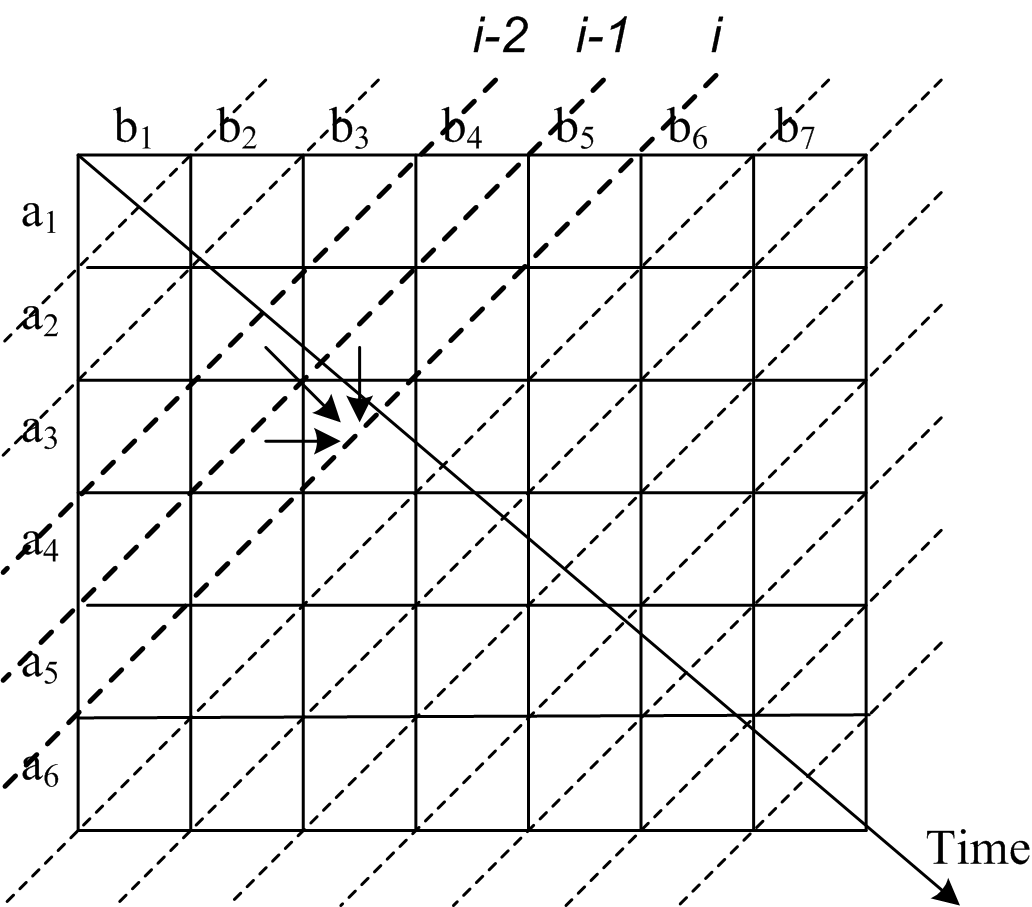
\includegraphics{graphics/smith-watermann-diagonal}
  \caption{Illustration of dependencies in the Smith-Watermann algorithm; diagonals are seen to be independent}
  \label{fig:sw-diagonal}  
  \end{figure}
%
In each row or column, the values of the $H$ matrix are defined
recursively, so there is no obvious inner or outer loop that is
parallel. However, the algorithm has a \indexterm{wavefront}
structure~\cite{Liu:cudasw2009}; see figure~\ref{fig:sw-diagonal} and
see section~\ref{sec:wavefront} for a further discussion on
wavefronts.

Assuming shared memory, we can split the $H$-matrix into blocks, and
apply the wavefront algorithm to the blocks: the blocks on each
diagonal can be processed in parallel. Inside each block, the
diagonals can be processed with \indextermbus{vector}{instructions}.

Each diagonal only needs two previous diagonals for its computation,
so the required amount of temporary space is linear in the input size.

\Level 0 {Suffix tree}

\url{http://homepage.usask.ca/~ctl271/857/suffix_tree.shtml}

For a word over some alphabet, a suffix is a contiguous substring of
the word that includes the last letter of the
word. A~\indexterm{suffix tree} is a data structure that contains all
suffices (of a word?). There are algorithms for constructing and
storing such trees in linear time, and searching with time linear in
the lenght of the search string. This is based on `edge-label
compression', where a suffix is stored by the indices of its first and
last character.

Example. The word `mississippi' contains the letters \emph{i,m,p,s},
so on the first level of the tree we need to match on these.
\[ 
\begin{array}{*{12}{c}}
i&m&p&s\\
\end{array}
\]
The `i' can be followed by `p' or~`s', so on the next level
we need to match on that.
\[ 
\begin{array}{*{12}{c}}
i& &m&p&s\\
p&s\\
\end{array}
\]
However, after `ip' is only one possibility, `ippi', 
and similarly after `is' the string `issi' uniquely
follows before we have another choice between `p' or~`s':
\[ 
\begin{array}{*{12}{c}}
i  &   &      &m&p&s\\
ppi&ssi\\
   &ppi&ssippi\\
\end{array}
\]
After we construct the full suffix tree we have a data structure
in which the time for finding a string of length~$m$ takes
time~$O(m)$.
Constructing the suffix tree for a string of length~$n$ 
can be done in time~$O(n)$.

Both 
\indexterm{genome alignment} and \indexterm{signature selection} can
be done with suffix trees.

